\documentclass[12pt]{article}
% pre\'ambulo

\usepackage{lmodern}
\usepackage[T1]{fontenc}
\usepackage[spanish,activeacute]{babel}
\usepackage{mathtools}
\usepackage{titlesec}
\usepackage{verbatim}
\usepackage{moreverb}
\usepackage{fancybox}
\usepackage{fancyhdr}
\usepackage{graphicx}
\usepackage{array}
\usepackage{enumerate}
\usepackage{multicol}
\usepackage{multirow}
\usepackage[dvipsnames]{xcolor}
\usepackage{amsfonts}
\usepackage{ulem}
\usepackage{array}
\usepackage[utf8]{inputenc}
%\usepackage[usenames]{color}

\newtheorem{defin}{Definición}

%% Figuras
\graphicspath{{./Imagenes/}}

\setlength{\textwidth}{18cm}   
\setlength{\evensidemargin}{0.5cm}
\setlength{\footskip}{1.5cm}
\setlength{\textheight}{22cm} 
\voffset -2cm
\hoffset -2cm
\pagestyle{plain}


\begin{document}
	
	
	\decimalpoint
	
	\renewcommand{\tablename}{Tabla}
	
	\fancyput(8.29cm,-11.436cm){
		\setlength{\unitlength}{1in}\hspace{-0.2cm}\fancyoval(7.7,10.4)}
	\thispagestyle{empty}
	\vspace*{\fill}
	\begin{center}
		{\huge (El título)\\\vspace{0.7cm}
	}\vspace{2cm} 
		{\Large por:}	\\\vspace{1cm} 
		{\Large (Nombre del alumno o alumna)\\}
		\vspace{6cm} 
	Profesor:\\
	Dr. José Daniel Castro Díaz
		
		
		
	\end{center}
	
	
	
	
	\vspace*{\fill}	
	
	\newpage
	\setcounter{page}{1}
	
	
	\newpage
	
	\section{Una sección}
Aquí escribe algo...
    \section{Otra sección}
Aquí también... usando las referencias. Por ejemplo, en la Figura \ref{Baleros} se observa una carretilla remachada. 
    
    	\begin{figure}[h]
		\centering
		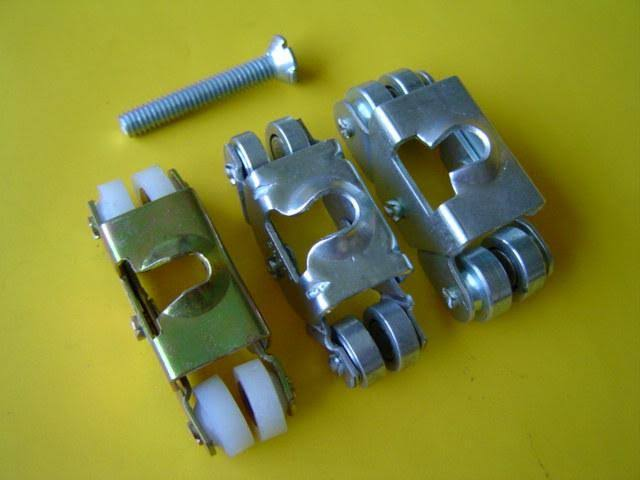
\includegraphics[width=10cm]{Ensamble}
		\caption{Carretillas remachadas con 2 balancines y 4 baleros}
		\label{Baleros}
	\end{figure}


    

	\end{document}